\subsection[cppyy]{The cppyy project}

\begin{frame}
  \frametitle{Automatic Python-C++ bindings}
  \begin{block}{The {\color{blue!50!white} \href{https://cppyy.readthedocs.io}{cppyy}} project}
    \begin{itemize}
    \item originated from the ROOT project
    \item still young, version 1.0 from Mid 2018
    \item but very active,  current version 2.1.0
    \item extremely powerful for interfacing \cpp and python
    \end{itemize}
  \end{block}
  \begin{block}{How it works}
    \begin{itemize}
    \item uses Just in Time compilation through {\color{blue!50!black} \href{https://github.com/vgvassilev/cling}{cling}}
      \begin{itemize}
      \item an interactive \cpp interpreter
      \end{itemize}
    \end{itemize}
  \end{block}
\end{frame}

\begin{frame}
  \frametitle{cppyy crash course(1)}
  Shamelessly copied from the cppyy documentation
  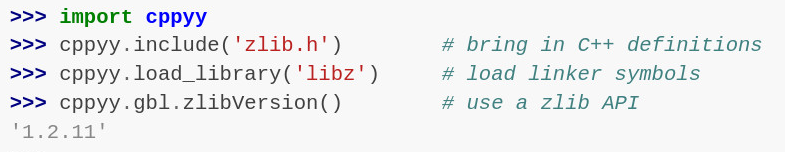
\includegraphics[width=.8\textwidth]{python/cppyy2.png}
  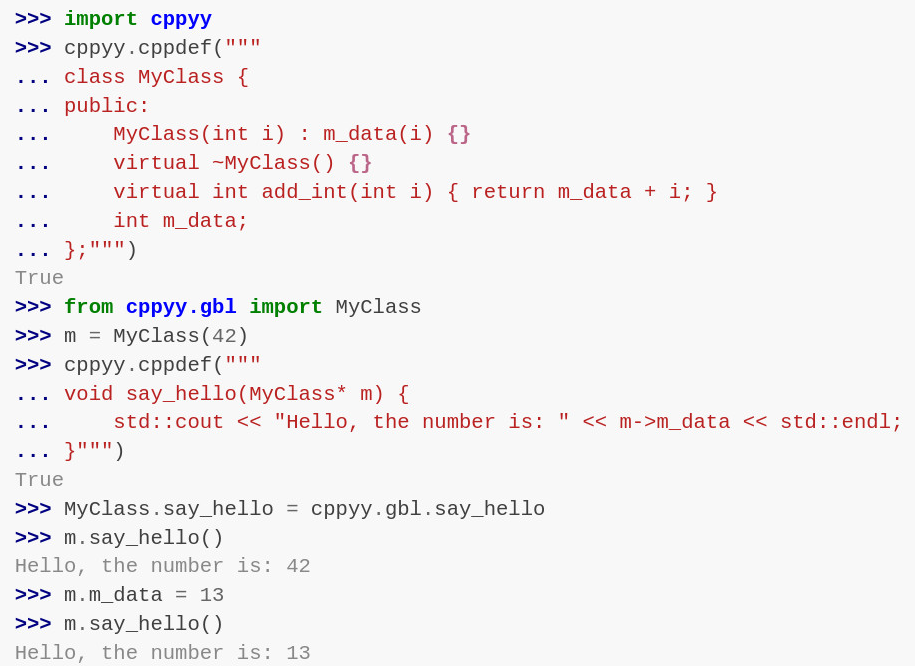
\includegraphics[trim={0 3.2cm 0 0},clip,width=\textwidth]{python/cppyy.png}
\end{frame}

\begin{frame}
  \frametitle{cppyy crash course(1)}
  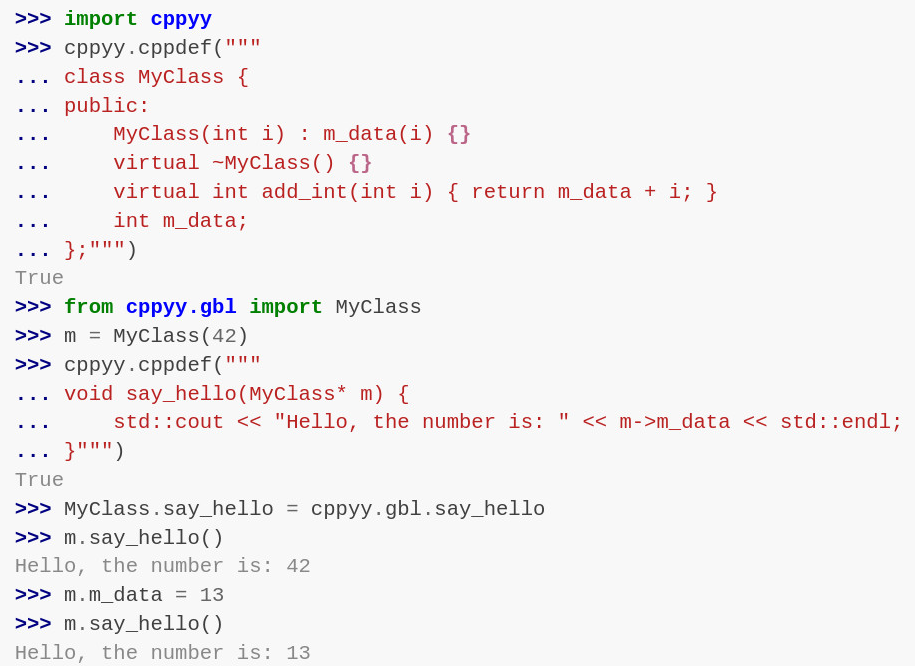
\includegraphics[trim={0 0 0 2.45cm},clip,width=\textwidth]{python/cppyy.png}
\end{frame}
